\chapter{Analytics Delivery and Visualisation}
\section{Multi-Channel Insight Delivery}
The platform exposes curated KPIs through multiple delivery channels tailored to stakeholder workflows:
\begin{itemize}
    \item \textbf{Power BI Premium} dashboards for merchandising and supply chain analysts with drill-through into SKU and vendor performance.
    \item \textbf{Tableau Server} storyboards targeted at executive leadership, emphasising strategic KPIs and scenario modelling.
    \item \textbf{Amazon QuickSight} embedded analytics for marketplace sellers, giving partners visibility into fulfilment and conversion metrics.
    \item \textbf{Responsive web portal} built with React and Tailwind CSS, updating every two minutes via WebSocket streams.
    \item \textbf{Automated communications} delivering PDF scorecards and Slack/Teams alerts triggered by KPI thresholds.
\end{itemize}

\section{KPI Catalogue}
A governed KPI catalogue ensures consistent definitions across channels. Table~\ref{tab:kpi} lists the headline metrics.

\begin{table}[H]
    \centering
    \caption{Headline KPIs and refresh characteristics}
    \label{tab:kpi}
    \begin{tabular}{p{4cm}p{5cm}p{3cm}p{2cm}}
        \toprule
        \textbf{KPI} & \textbf{Description} & \textbf{Source Models} & \textbf{Refresh} \\
        \midrule
        Net Revenue & Gross revenue minus discounts, refunds, taxes & fact\_order, dim\_channel & 2 min \\
        Conversion Rate & Sessions to orders ratio & fact\_order, fact\_session & 2 min \\
        Fulfilment SLA & Orders delivered within promised window & fact\_shipment & 5 min \\
        Return Rate & Returns initiated vs dispatched orders & fact\_order, fact\_returns & 10 min \\
        CSAT Index & Weighted customer satisfaction score & fact\_support\_case & 2 min \\
        Inventory Risk & Days of cover vs forecast demand & fact\_inventory, dim\_product & 15 min \\
        \bottomrule
    \end{tabular}
\end{table}

\section{Performance Benchmarking}
Latency reductions were validated through controlled tests comparing legacy and new pipelines. Figure~\ref{fig:latency} illustrates the improvement.

\begin{figure}[H]
    \centering
    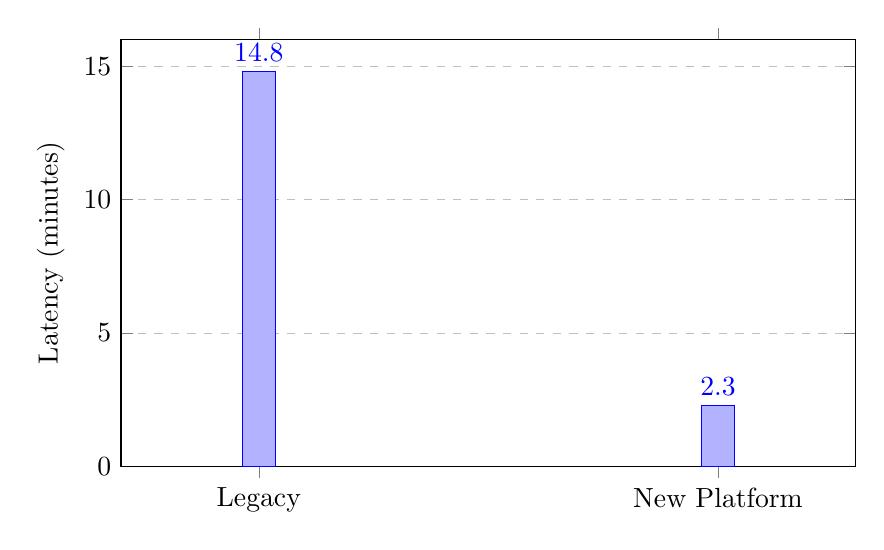
\begin{tikzpicture}
        \begin{axis}[
            ybar=6pt,
            width=0.9\textwidth,
            height=7cm,
            bar width=12pt,
            ylabel={Latency (minutes)},
            symbolic x coords={Legacy,New Platform},
            xtick=data,
            nodes near coords,
            nodes near coords align={vertical},
            ymin=0,
            ymax=16,
            ymajorgrids=true,
            grid style=dashed,
            enlarge x limits=0.3,
            fill=blue!50
        ]
            \addplot coordinates {(Legacy,14.8) (New Platform,2.3)};
        \end{axis}
    \end{tikzpicture}
    \caption{Median KPI refresh latency before and after implementation}
    \label{fig:latency}
\end{figure}

\section{Dashboard Design Principles}
\begin{itemize}
    \item \textbf{Visual hierarchy} emphasises alerts, exceptions, and trend inflections using colour-coded thresholds.
    \item \textbf{Accessibility} adheres to WCAG 2.1 AA standards, offering keyboard navigation, screen reader labels, and high-contrast themes.
    \item \textbf{Self-service exploration} via drill-through, natural language queries, and embedded metadata tooltips.
    \item \textbf{Feedback loops} collect user comments directly within dashboards, feeding backlog refinement.
\end{itemize}

\section{Distribution and Automation}
Daily distribution includes automated PDF snapshots stored in Amazon S3 and emailed to regional leads. Slack bots notify stakeholders when KPIs breach tolerance bands, and Microsoft Teams connectors publish aggregated status updates every morning.
